\documentclass[a4paper]{scrartcl}
\usepackage[sexy]{evan}
\usepackage{graphicx}
\usepackage{wrapfig}
\graphicspath{ {./build/} }

\author{Mckinley Xie}
\title{\LaTeX{} Practice}

\begin{document}
\maketitle

Hello! I'm Mckinley! This is a bunch of words and two images and two problems.

I'll be using the \texttt{evan.sty} style file by Evan Chen since it looks really nice.
You can find it \href{https://github.com/vEnhance/dotfiles/blob/main/texmf/tex/latex/evan/evan.sty}{here}.

You can find the the source to this \href{https://github.com/MckinleyX/ib-math-handouts/blob/master/practice.tex}{here}.

Here goes!


\begin{wrapfigure}{r}{0.25\textwidth}
	\centering
	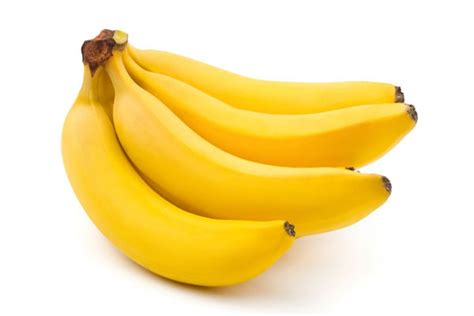
\includegraphics[width=0.25\textwidth]{banana}
\end{wrapfigure}

I like competitive math. On last year's AMC 12A I got a score of 118.5 (though, somehow, my AMC 10B score was significantly worse) and on the AIME I got a score of 7. I'm hoping to qualify for USAMO this year. My favorite subject is (by far) combinatorics, and my weakest is probably geometry. (I'm not too sure what I want to do for my IA/EE, I think something about extremal graph theory, maybe Sperner's theorem or something, but that might be over my head.) I have an image of a banana here since... uhh... I dunno.

\begin{wrapfigure}{l}{0.15\textwidth}
	\centering
	
\includegraphics[width=0.15\textwidth]{tux}
\end{wrapfigure}
\leavevmode

At the moment I'm also working on a couple of handouts for Math HL since some people seem to be confused, they can currently be found at \url{https://mckinleyx.github.io}. At the moment I'm trying to write something about modular arithmetic, but that may change on my whim.

In other news, I also do Linux! Both my laptop and my desktop are currently running bspwm on Arch Linux, and my current \LaTeX{} setup is Vim + \href{https://github.com/lervag/vimtex}{VimTeX} + texlive. 

\newpage
Here are my two problems!

\begin{example*}
	[2020 IMO Shortlist C1]
	Let $n$ be a positive integer. Find the number of permutations $a_1, a_2, \dots a_n$ of the sequence $1,2,\dots n$ satisfying 
	\[a_1 \leqslant 2a_2 \leqslant 3a_3 \leqslant \dots \leqslant na_n\]
\end{example*}
\begin{proof}
	We claim that the number of permutations is the $n^\text{th}$ fibonacci number, $F_n$, defined as $F_0 = F_1 = 1, F_n = F_{n-2} + F_{n-1}$.
	\begin{claim*}
		If $a_i = n$, then $i \geq n-1$.
	\end{claim*}
	\begin{proof}
	Suppose that $a_i = n$. Then $\{a_{i+1} \dots a_n\}$ must be a permutation of $\{ i, i+1, \dots n-1\}$. $i$ must be at location $n$, which implies that $in = (i+1)a_{n+1} = \cdots = ni$, which is clearly impossible for $i < n-1$.
	\end{proof}

	To finish we will use strong(-ish?) induction. Clearly the claim is true for $n=1$ and $n=2$. Now, suppose the claim is true for some $n-2$ and $n-1$. Now, we will use caeswork on the position of $n$.

	\textbf{Case 1.} If $a_n = n$ the number of permutations satisfying the condition is equivalent to $F_{n-1}$ since $n^2$ is greater than any other term in the inequality.

	\textbf{Case 2.} If $a_{n-1} = n$, then $na_n \geq n(n-1) \implies a_{n} \geq n-1$, and now $n(n-1)$ is greater than or equal to any other terms in the inequality, so the number of permutations in this case is $F_{n-2}$.

	The sum of these are $F_{n-1} + F_{n-2} = F_n$ and we are done.
	
\end{proof}

\begin{verbatim}
	\begin{example*} %this is from evan.sty
		[2020 IMO Shortlist C1]
		Let $n$ be a positive integer. 
		Find the number of permutations 
		$a_1, a_2, \dots a_n$ of the sequence $1,2,\dots n$ 
		satisfying 
		\[a_1 \leqslant 2a_2 \leqslant 3a_3 \leqslant \dots \leqslant na_n\]
	\end{example*}

	\begin{proof} %also from evan.sty
		We claim that the number of permutations
		is the $n^\text{th}$ fibonacci number, $F_n$, 
		defined as $F_0 = F_1 = 1, F_n = F_{n-2} + F_{n-1}$.
		\begin{claim*} % evan.sty
			If $a_i = n$, then $i \geq n-1$.
		\end{claim*}
		\begin{proof}
		Suppose that $a_i = n$. 
		Then $\{a_{i+1} \dots a_n\}$ must be a permutation of 
		$\{ i, i+1, \dots n-1\}$.
		$i$ must be at location $n$,
		which implies that $in = (i+1)a_{n+1} = \cdots = ni$, 
		which is clearly impossible for $i < n-1$.
		\end{proof}

		To finish we will use strong(-ish?) induction.
		Clearly the claim is true for $n=1$ and $n=2$.
		Now, suppose the claim is true for some $n-2$ and $n-1$.
		Now, we will use casework on the position of $n$.

		\textbf{Case 1.} If $a_n = n$ the number of permutations 
		satisfying the condition is equivalent to $F_{n-1}$ 
		since $n^2$ is greater than any other term in the inequality.

		\textbf{Case 2.} If $a_{n-1} = n$, then 
		$na_n \geq n(n-1) \implies a_{n} \geq n-1$, 
		and now $n(n-1)$ is greater than or equal to 
		any other terms in the inequality, 
		so the number of permutations in this case is $F_{n-2}$.

		The sum of these are $F_{n-1} + F_{n-2} = F_n$ and we are done.
	\end{proof}
\end{verbatim}


\begin{example*}
	[Erd\H{o}s-Szekeres]
	Prove that, in a sequence of $mn + 1$ distinct integers, $\exists$ either an increasing subsequence of length $m+1$ or a decreasing subsequence of $n+1$.
\end{example*}
\begin{proof}
	Let our sequence be $a_1, a_2, \cdots a_{mn+1}$.

	Let $L(x)$ (similarly, $L'(x)$) denote the length of the longest increasing (similarly, decreasing) subsequence ending at $a_x$.

	Now, consider $x$ and $y$ such that $1 \leq x < y \leq mn + 1$. Because $a_y$ is either greater than or less than $a_x$, either $L(y) > L(x)$ or $L'(y) > L'(x)$, since we can always create a larger subsequence of one kind by appending $a_y$ to a subsequence ending at $a_x$.

	Because this is true $\forall x,y$ in the given range, then each $a_x$ corresponds to a unique ordered pair $(L(x), L'(x))$.

	Now, suppose our claim is not true, and that there do not exist such subsequences. Then $\forall x $ such that $1 \leq x \leq mn+1$, $1 \leq L(x) \leq m$ and $1 \leq L'(x) \leq n$. However, observe that there are only $mn$ ordered pairs $(L(x), L'(x))$ satisfying that condition, so by the pigeonhole principle such a subsequence exists, and we are done.

\end{proof}
\begin{verbatim}
\begin{example*}
	[Erd\H{o}s-Szekeres]
	Prove that, in a sequence of $mn + 1$ distinct integers, 
	$\exists$ either an increasing subsequence of length $m+1$ 
	or a decreasing subsequence of $n+1$.
\end{example*}
\begin{proof}
	Let our sequence be $a_1, a_2, \cdots a_{mn+1}$.

	Let $L(x)$ (similarly, $L'(x)$) denote the length of the 
	longest increasing (similarly, decreasing) subsequence ending at $a_x$.

	Now, consider $x$ and $y$ such that $1 \leq x < y \leq mn + 1$. 
	Because $a_y$ is either greater than or less than $a_x$, 
	either $L(y) > L(x)$ or $L'(y) > L'(x)$, 
	since we can always create a larger subsequence of one kind 
	by appending $a_y$ to a subsequence ending at $a_x$.

	Because this is true $\forall x,y$ in the given range, 
	each $a_x$ corresponds to a unique ordered pair $(L(x), L'(x))$.

	Now, suppose our claim is not true, 
	and that there do not exist such subsequences. 
	Then $\forall x $ such that $1 \leq x \leq mn+1$,
	$1 \leq L(x) \leq m$ and $1 \leq L'(x) \leq n$. 
	However, observe that there are only $mn$ ordered pairs $(L(x), L'(x))$ 
	satisfying that condition, 
	so by the pigeonhole principle such a subsequence exists, 
	and we are done.
\end{proof}
\end{verbatim}

\end{document}
